\documentclass[portrait,color=UCLmidgreen,margin=1.5cm,bannerheight=8cm,logoheight=2.5cm]{uclposter}
\usepackage{tikz}
\usepackage[scaled=1.2]{helvet}
\renewcommand\familydefault{\sfdefault} 
\usepackage[T1]{fontenc}
\usepackage{tcolorbox}

\title{Performance characterisation of 8-bit RISC and OISC architectures}

\author{Mindaugas Jarmolovicius}

%\affil[1]{UCL Electronic And Electrical Engineering}

\begin{document}

%\tikz\node[opacity=0.3,inner sep=0]{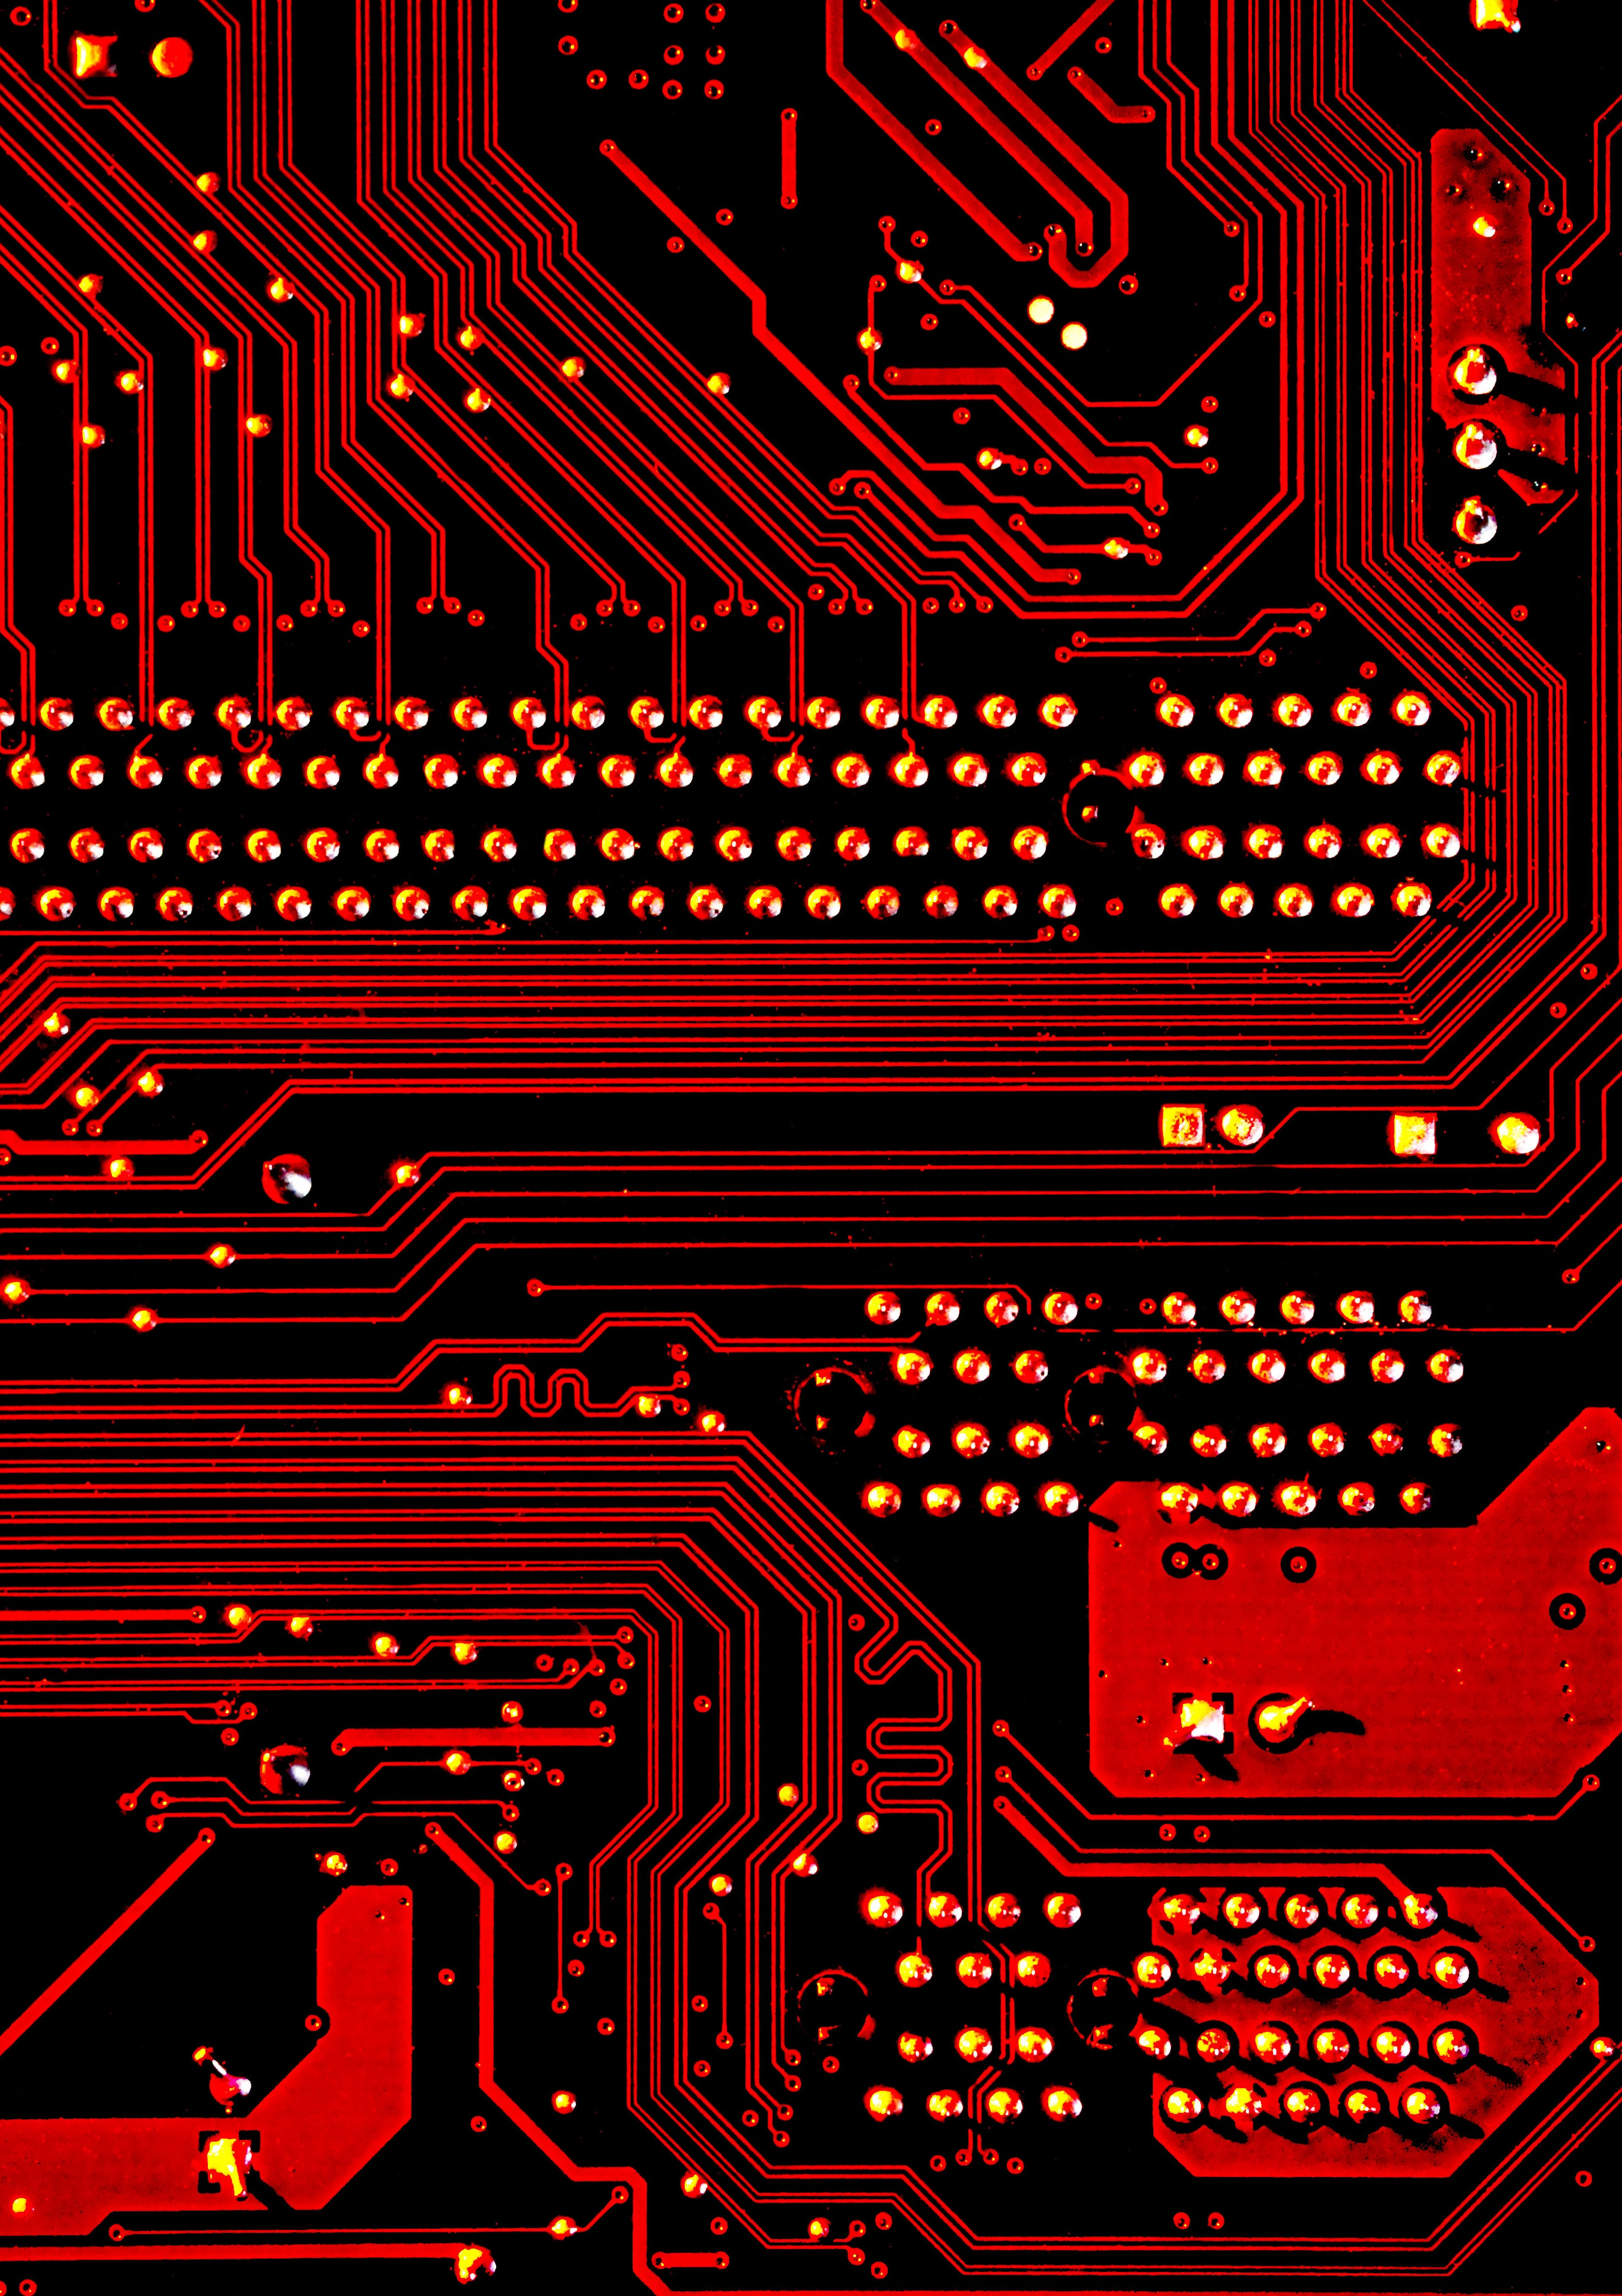
\includegraphics[height=\paperheight,width=\paperwidth]{background.jpg}}
%\tikz[remember picture,overlay] \node[opacity=0.3,outer sep=0pt] at (current page.center){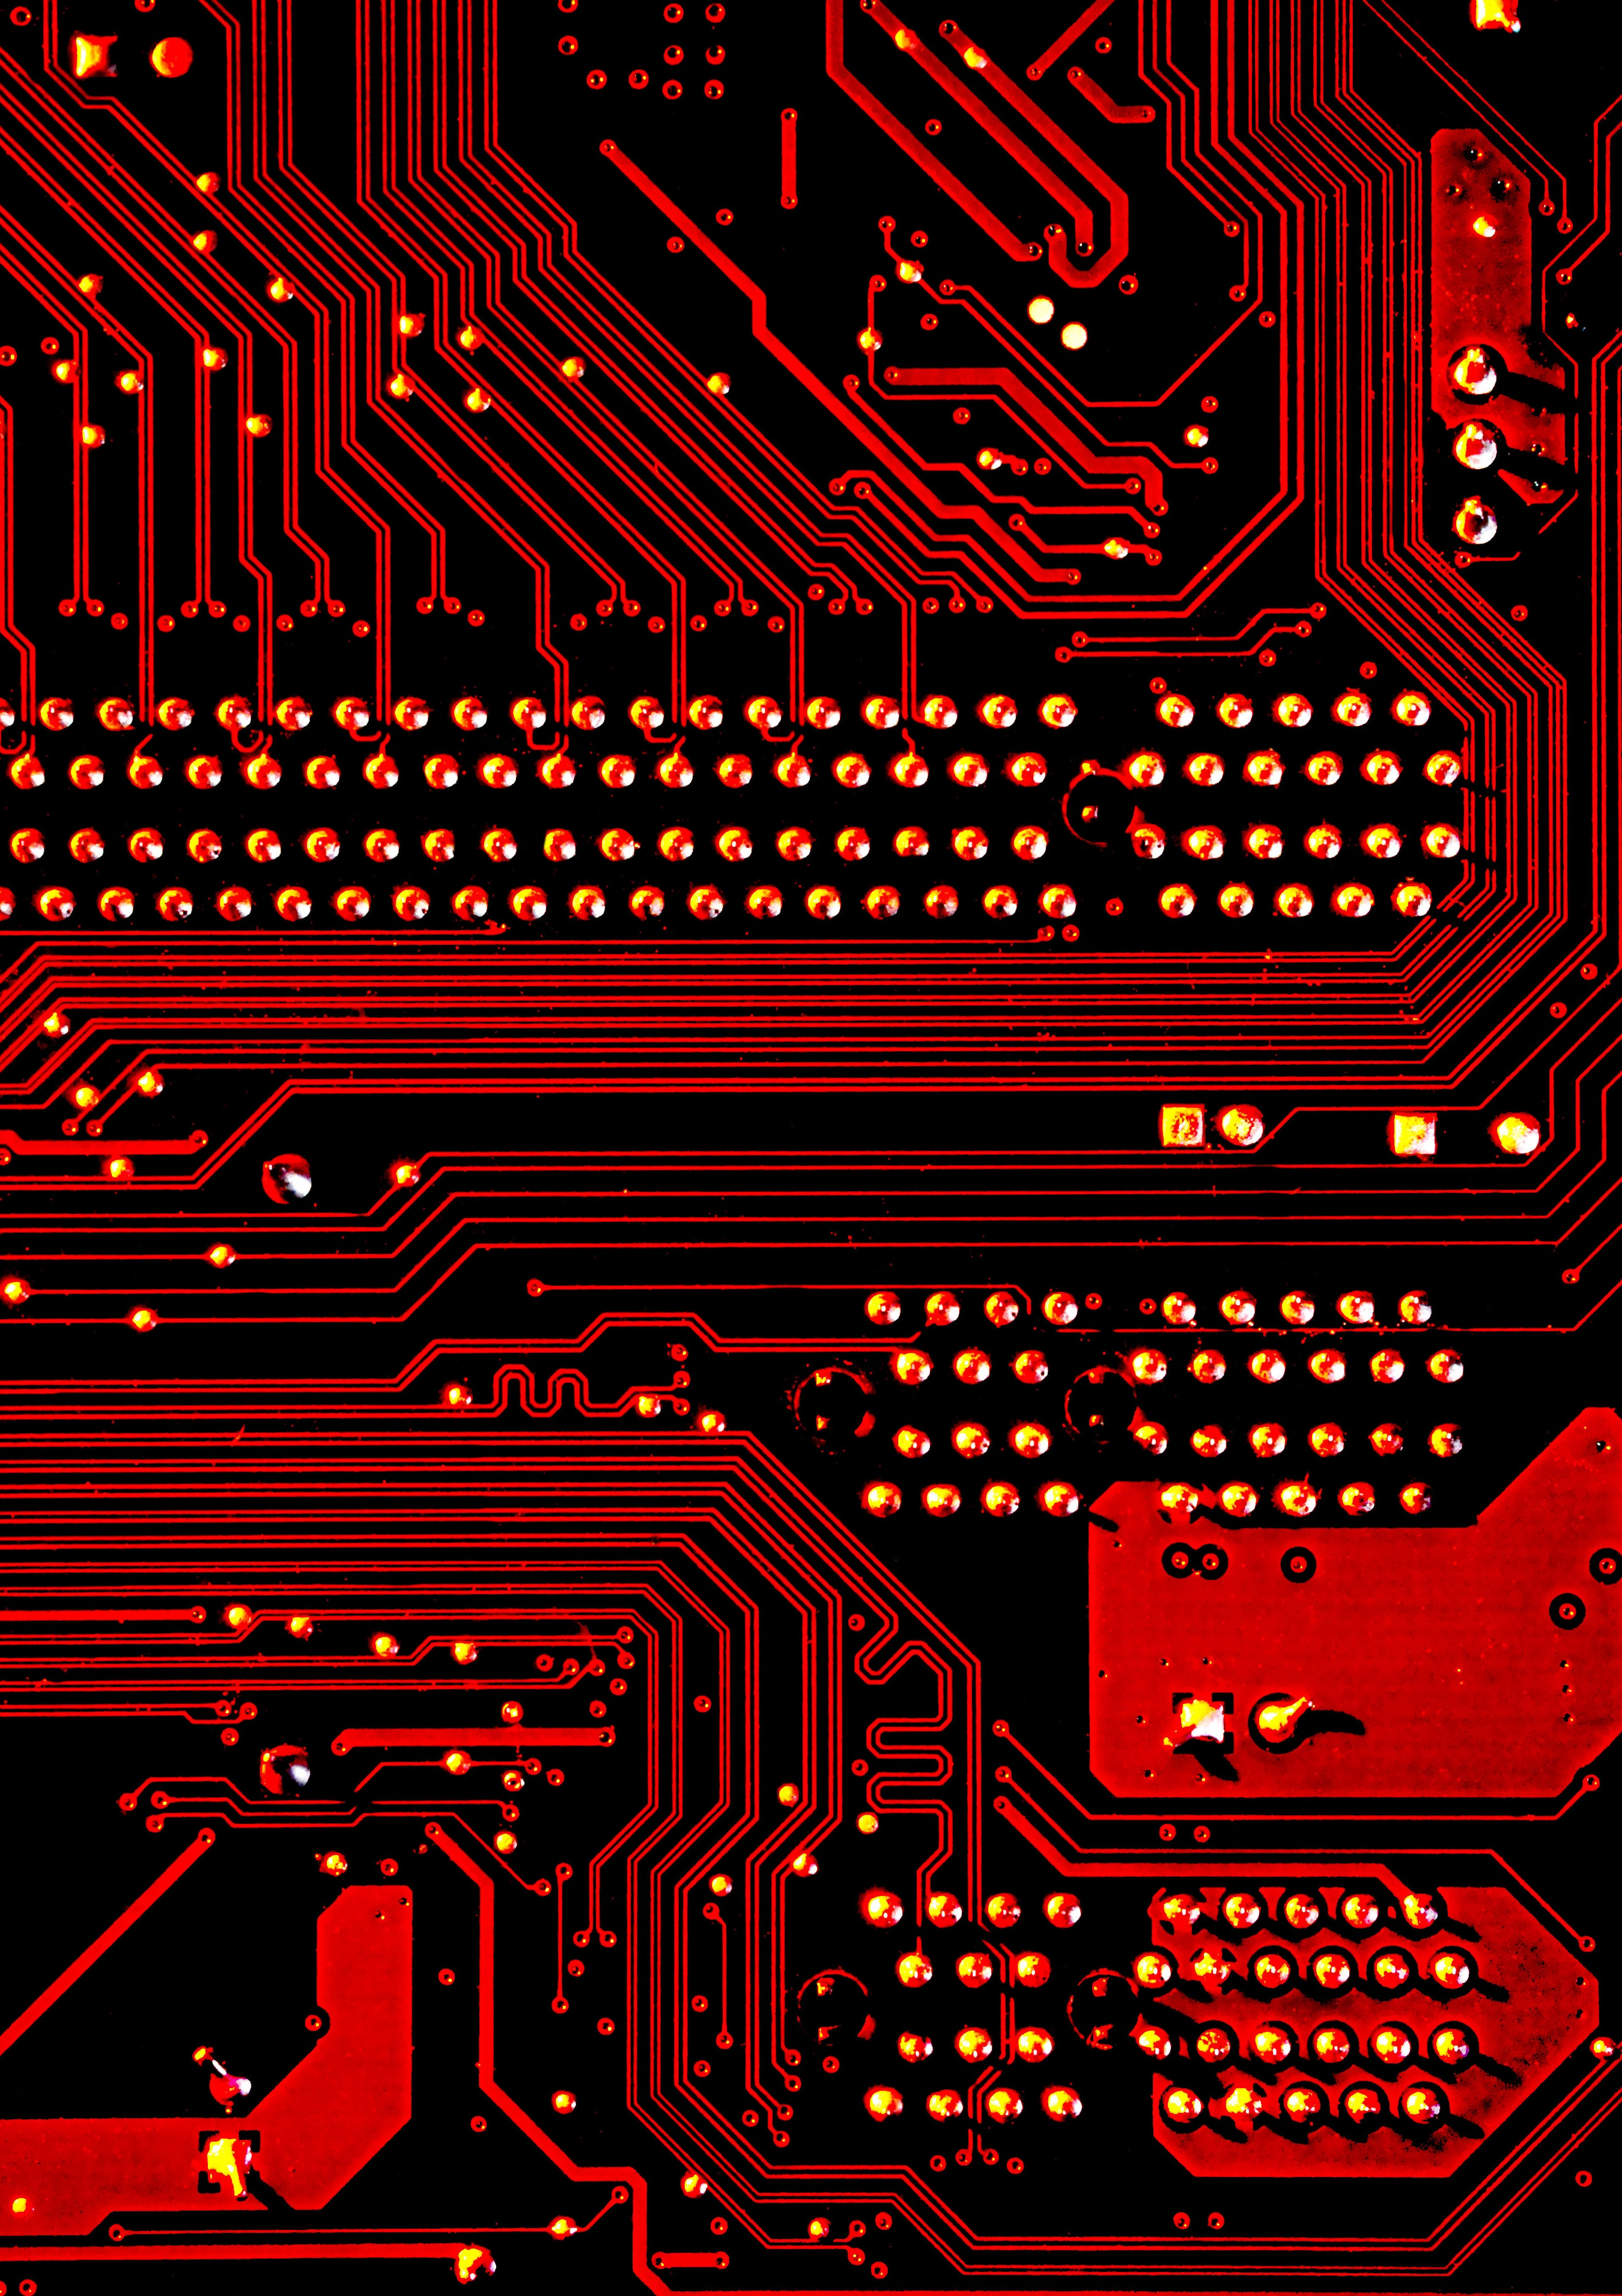
\includegraphics[width=\paperwidth,height=\paperheight]{background.jpg}};

\maketitle
\tcbset{colframe=UCLmidgreen,center title,fonttitle=\bfseries\Large,toptitle=1.5mm,bottomtitle=1.5mm,boxrule=0.8mm,sharp corners}
\begin{tcolorbox}[title=Introduction]
	
This is a bunch of text for introductions that describes project, what it is about and that it compares RISC versus OISC architectures. Also motivation and academic papers.
\end{tcolorbox}


\begin{multicols}{2}
	
\begin{tcolorbox}[title=RISC Architecture]
	
	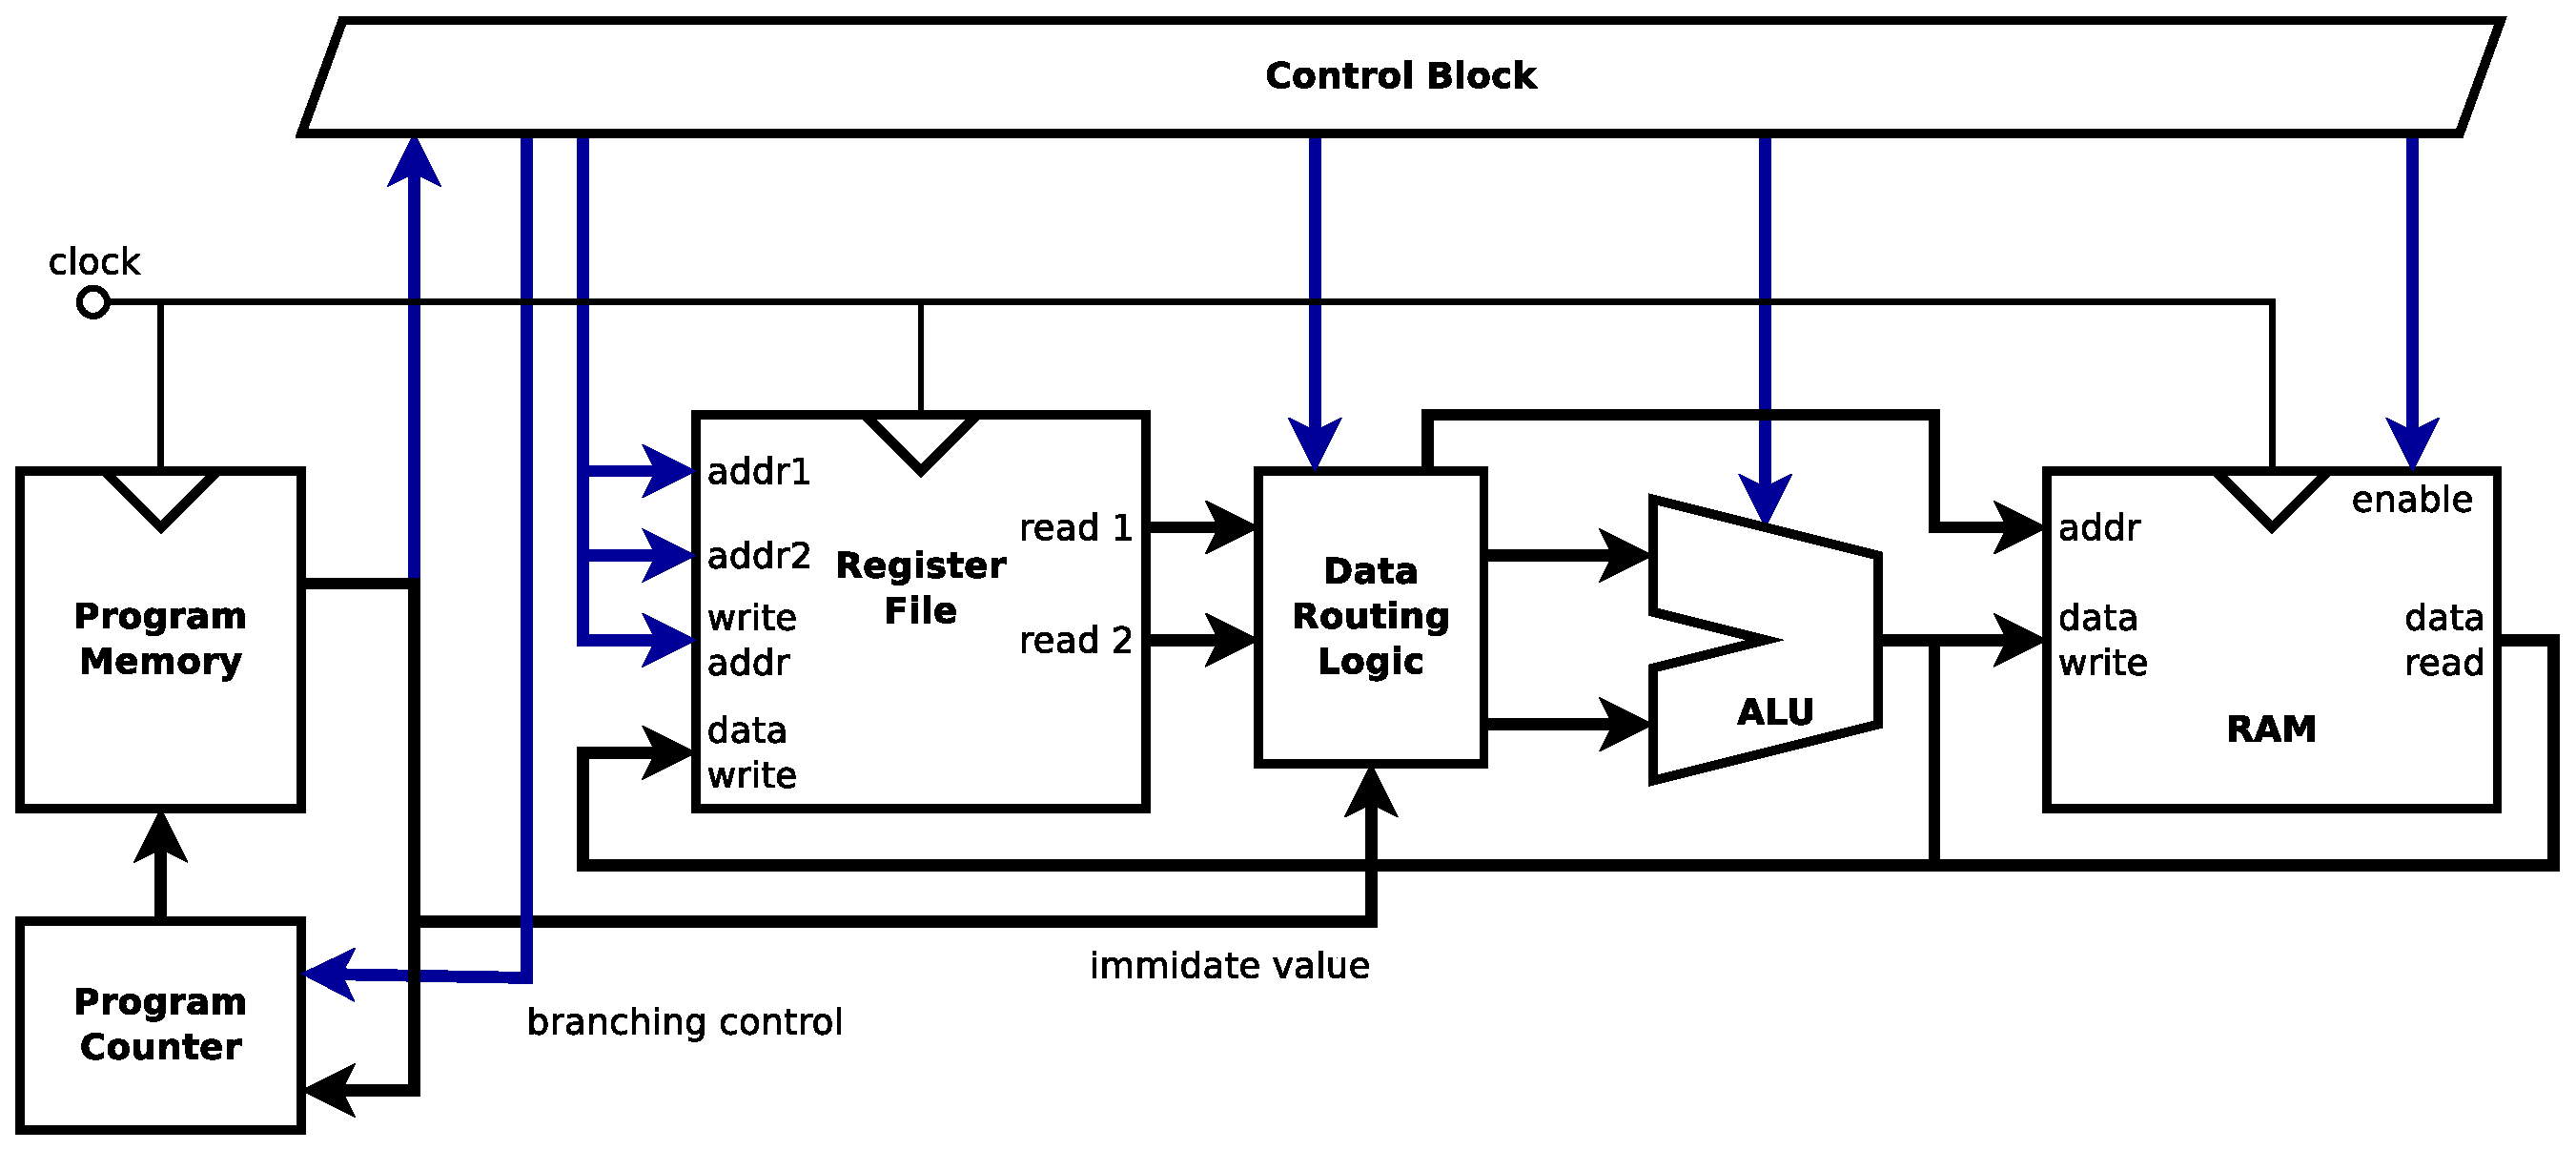
\includegraphics[width=\linewidth]{../resources/risc.eps}
	\centering
	\textit{Figure 1: RISC architecture general block diagram}
	

	
	\begin{description}
		\item[$\bullet$] 45 Instructions
		\item[$\bullet$] 
	\end{description}


	
	\begin{description}
		\item[$\bullet$] Bunch of instructions
		\item[$\bullet$] Efficient instruction space
		\item[$\bullet$] Generally easy to use but damn to low number of registers.
		\item[$\bullet$] Needs optimisation.
	\end{description}
\end{tcolorbox}

%\begin{highlightbox}[UCLdarkblue!20!white]
%\end{highlightbox}

\columnbreak



\begin{tcolorbox}[title=OISC Architecture]
	
	
	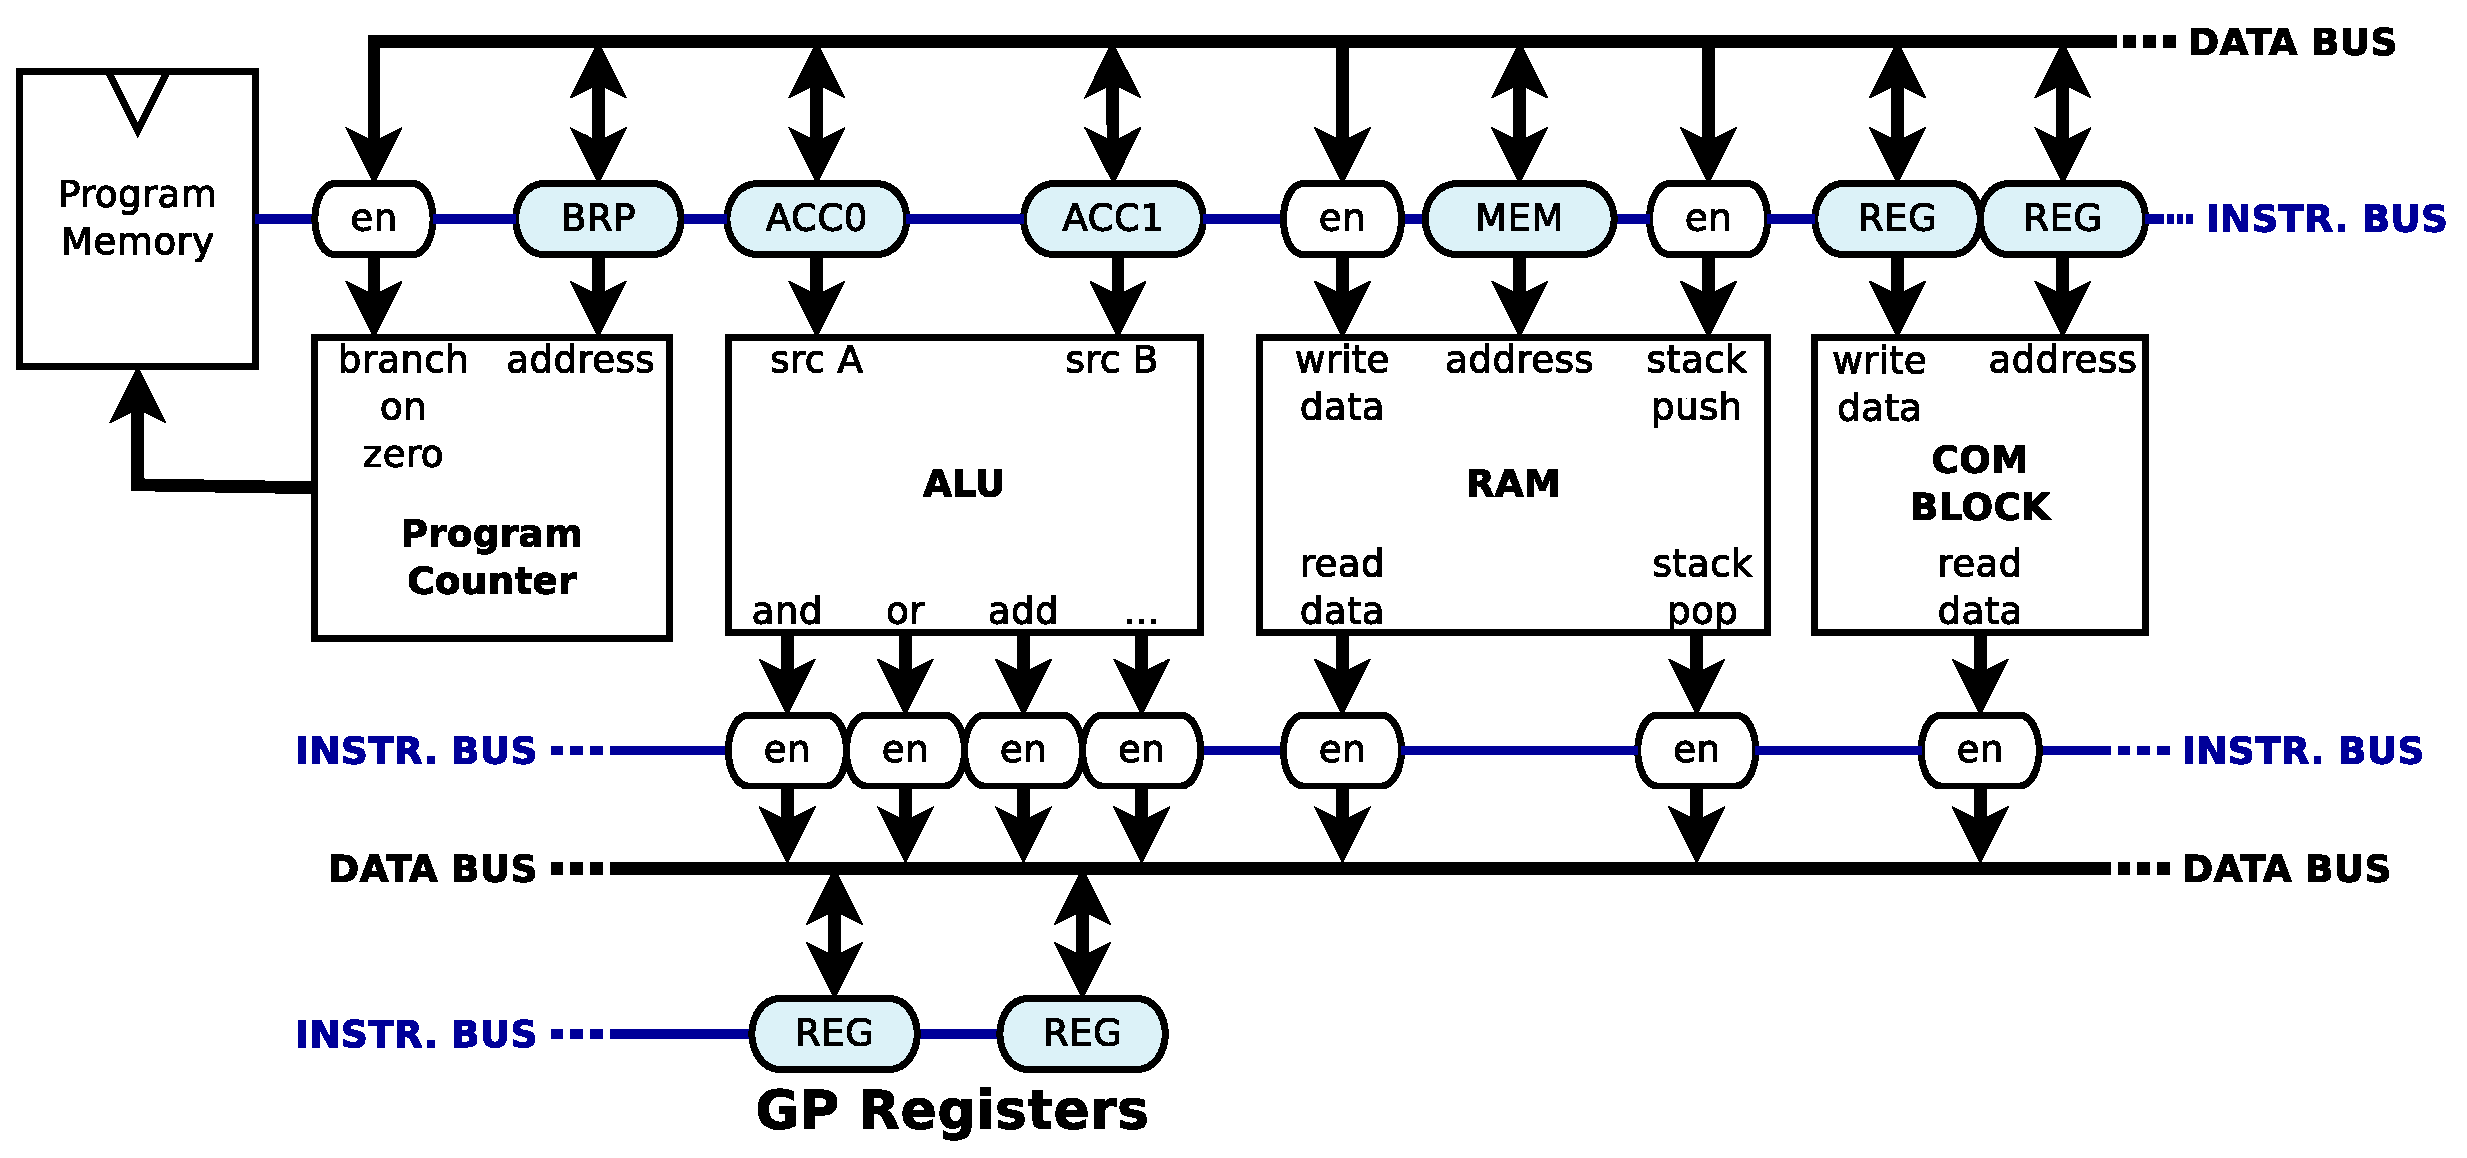
\includegraphics[width=\linewidth]{../resources/oisc.eps}
	\centering
	\textit{Figure 2: OISC architecture general block diagram}
\end{tcolorbox}
\begin{tcolorbox}[detach title]
	\definecolor{c1}{HTML}{ff7568} 
	\definecolor{c2}{HTML}{8cbfff} 
	\definecolor{c3}{HTML}{a6ddb7} 
	\textbf{Machine code}\\
	OISC instruction are fixed 13bit width, 1 bit to set source as immediate value, 4bits for destination address and 8bit for source or immediate.
	\\
	\begin{gather*}
	\scalebox{0.8}{bit index:}
	\underbrace{\colorbox{c1}{0}}_\text{imm.}
	\underbrace{
		\colorbox{c2}{1}\,
		\colorbox{c2}{2}\,
		\colorbox{c2}{3}\,
		\colorbox{c2}{4}\,
	}_\text{destination}
	\underbrace{
		\colorbox{c3}{5}\,
		\colorbox{c3}{6}\,
		\colorbox{c3}{7}\,
		\colorbox{c3}{8}\,
		\colorbox{c3}{9}\,
		\colorbox{c3}{10}\,
		\colorbox{c3}{11}\,
		\colorbox{c3}{12}
	}_\text{source}
	\end{gather*} 
	\\
	\textbf{Total number of:}
	\begin{description}
		\item[$\bullet$] 15 Destination addresses
		\item[$\bullet$] 41 Source addresses
	\end{description}
\end{tcolorbox}
\begin{tcolorbox}[detach title]
	\begin{description}
		\item[$\bullet$] Only one instruction
		\item[$\bullet$] Not so efficient instruction space
		\item[$\bullet$] Takes forever to write in assembly
		\item[$\bullet$] Takes no time to improve. It just asking for more data buses!
	\end{description}

\end{tcolorbox}

\end{multicols}


\begin{tcolorbox}[title=Results]
	Following functions have been implemented in assembly:
	\begin{description}
		\item[$\bullet$] Print ASCII, Binary, Hexadecimal and Decimal (8 and 16bit)
		\item[$\bullet$] 16bit multiplication
		\item[$\bullet$] 16bit division 
		\item[$\bullet$] 16bit modulus
		\item[$\bullet$] Sieve of Atkins (prime number calculator)
	\end{description}
\end{tcolorbox}


\begin{tcolorbox}[title=Future work]
Explain future work, experiments, oisc improvements.
\end{tcolorbox}


\end{document}
